\chapter{De las integrales de camino a los propagadores y vértices}

Antes de pasar al inventario de partículas y sus interacciones, conviene aclarar la construcción central. Un lagrangiano no solo codifica las ecuaciones clásicas de los campos. A través de la integral de camino también proporciona amplitudes para que las partículas se propaguen, se dividan, se unan y dispersen. Esta es la vía más directa de la teoría cuántica de campos a los diagramas de Feynman.

\section{Acción mínima para partículas y campos}

La integral de camino de Feynman es la contraparte cuántica del principio de acción mínima. Comencemos con una partícula newtoniana ordinaria, cuyo lagrangiano depende de sus coordenadas y velocidades,
\begin{equation}
\mathcal{L}=\mathcal{L}(x,\dot{x}),
\end{equation}
y cuya acción asignada a una trayectoria es
\begin{equation}
S[x]=\int \mathcal{L}(x,\dot{x})\,dt.
\end{equation}
Toda trayectoria posible entre dos puntos del espacio-tiempo tiene una acción, satisfaga o no las ecuaciones de Newton. La trayectoria clásica se distingue porque la acción es estacionaria. En el lenguaje tradicional de la ``acción mínima'', la acción se minimiza, aunque «estacionaria» es la afirmación más general. La condición de estacionariedad da las ecuaciones diferenciales clásicas del movimiento.

\begin{figure}[htbp]
\centering
\includegraphics[width=0.72\textwidth]{lecture_10_figure_02.png}
\caption{Integral de acción para la trayectoria de una partícula.}
\lectureframe{00:02:14}
\end{figure}

La misma estructura se aplica a un campo clásico. Denotemos genéricamente todos los campos por \(\phi\). La densidad lagrangiana local de un campo puede depender de los campos y de sus derivadas espaciales y temporales:
\begin{equation}
\mathcal{L}
=\mathcal{L}\!\left(\phi,\frac{\partial\phi}{\partial x^\mu}\right)
=\mathcal{L}(\phi,\partial_\mu\phi).
\end{equation}
La relatividad exige que \(\mathcal{L}\) se transforme como un escalar de Lorentz. Sujeta a este requisito, las combinaciones escalares construidas a partir de los campos y sus derivadas proporcionan los posibles términos del lagrangiano.

\begin{figure}[htbp]
\centering
\includegraphics[width=0.62\textwidth]{lecture_10_figure_03.png}
\caption{Dependencia del lagrangiano de campo respecto del campo y sus derivadas espacio-temporales.}
\lectureframe{00:04:09}
\end{figure}

Para un campo, la acción se integra sobre una región del espacio-tiempo:
\begin{equation}
S[\phi]=\int_{\Omega} d^4x\,\mathcal{L}(\phi,\partial_\mu\phi),
\qquad
d^4x=dt\,dx\,dy\,dz.
\end{equation}
La acción de una partícula es una integral sobre el tiempo a lo largo de un camino. La acción del campo es la integral de la densidad lagrangiana en toda una región del espacio-tiempo.

El análogo de fijar los extremos del camino de una partícula consiste en prescribir la configuración completa del campo en una hipersuperficie de tiempo inicial y en otra de tiempo final. Si el campo inicial es \(\phi_{\mathrm{i}}(\mathbf{x})\) y el final es \(\phi_{\mathrm{f}}(\mathbf{x})\), un campo interpolante ocupa toda la franja entre ambas. Cuando los datos de frontera admiten una solución clásica interpolante, esa solución es un punto estacionario de la acción con las configuraciones de frontera fijas.
\editorialnote{No toda pareja de configuraciones completas del campo en dos hipersuperficies de tiempo admite una solución clásica. Por tanto, la afirmación de acción estacionaria se restringe a los datos de frontera para los que existe una solución interpolante.}

La geometría es la contraparte, en la teoría de campos, del camino de una partícula.\footnote{La franja espacio-temporal se reconstruye a partir del diagrama de aproximadamente 00:04:29.}
\begin{figure}[htbp]
\centering
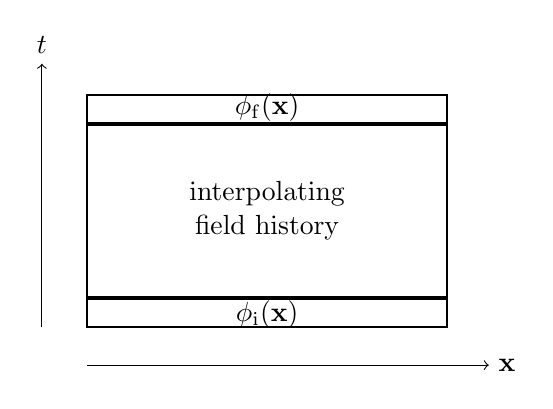
\begin{tikzpicture}[scale=0.88]
\draw[->] (-0.65,0) -- (-0.65,3.8) node[above] {$t$};
\draw[->] (0,-0.55) -- (5.8,-0.55) node[right] {$\mathbf{x}$};
\draw[thick] (0,0) rectangle (5.2,3.35);
\draw[very thick] (0,0.42) -- (5.2,0.42);
\draw[very thick] (0,2.93) -- (5.2,2.93);
\node at (2.6,0.18) {$\phi_{\mathrm{i}}(\mathbf{x})$};
\node at (2.6,3.17) {$\phi_{\mathrm{f}}(\mathbf{x})$};
\node[align=center] at (2.6,1.68) {interpolating\\field history};
\end{tikzpicture}
\caption{Configuraciones inicial y final del campo que delimitan una región del espacio-tiempo.}
\end{figure}

\begin{classroomqa}
\lecturetimestamp{00:07:34}
\audiencequestion{¿Puede un campo volver a tomar el mismo valor?}
\lecturerresponse{Sí. Nada impide que un campo vuelva a tomar un valor anterior, del mismo modo que nada impide que la coordenada de una partícula vuelva a una posición anterior.}
\end{classroomqa}

\begin{classroomqa}
\lecturetimestamp{00:07:46}
\audiencequestion{¿Por qué hablar de sucesos del espacio-tiempo o de una trayectoria si los datos de frontera son valores del campo?}
\lecturerresponse{El camino de la partícula se sustituye por una historia del campo. Cada extremo en el espacio de campos es el campo completo en una hipersuperficie de tiempo elegida, y una historia especifica el campo en cada punto de la región del espacio-tiempo entre ambas hipersuperficies.}
\end{classroomqa}

Exigir que la acción del campo interpolante sea estacionaria produce ecuaciones diferenciales parciales. Según los campos y el lagrangiano, estas incluyen ecuaciones como las de Maxwell y, para una acción gravitatoria, las ecuaciones de Einstein. Aquí no hace falta desarrollar la derivación variacional; la secuencia importante es
\begin{equation}
\mathcal{L}
\longrightarrow
S[\phi]
\longrightarrow
\text{classical field equations}.
\end{equation}

\section{La suma de Feynman sobre caminos de partículas}

La mecánica cuántica sustituye la pregunta de qué trayectoria ocurre por una pregunta sobre amplitudes. Imaginemos que se inyecta una partícula en \((x,t)\), se cierran los ojos un rato y luego se enciende un detector en \((x',t')\). La amplitud
\begin{equation}
\mathcal{A}(x,t;x',t')
\end{equation}
es un número complejo. Su módulo al cuadrado es la probabilidad:
\begin{equation}
\begin{aligned}
P(x,t;x',t')
&=\left|\mathcal{A}(x,t;x',t')\right|^2\\
&=\mathcal{A}(x,t;x',t')
\mathcal{A}(x,t;x',t')^*.
\end{aligned}
\end{equation}

La regla de Feynman asigna una acción a cada camino posible y le asocia la fase
\begin{equation}
\exp\!\left(-\frac{i}{\hbar}S[x]\right)
=
\exp\!\left[-\frac{i}{\hbar}\int \mathcal{L}(x,\dot{x})\,dt\right].
\end{equation}

\begin{figure}[htbp]
\centering
\includegraphics[width=0.70\textwidth]{lecture_10_figure_04.png}
\caption{Fase compleja asociada a un camino de partícula.}
\lectureframe{00:11:52}
\end{figure}

El factor de \(\hbar\) es necesario para que el exponente sea adimensional.\footnote{En 00:11:52, lo escrito en la pizarra se interpreta naturalmente como \(e^{-i\int\mathcal{L}\,dt}\); el factor de \(\hbar\) se añade oralmente en 00:12:02.} La amplitud de transición es la suma de estas fases sobre todos los caminos posibles que conectan los extremos:
\begin{equation}
\mathcal{A}(x,t;x',t')
=
\sum_{\substack{\text{paths }x(\tau)\\(x,t)\rightarrow(x',t')}}
\exp\!\left(-\frac{i}{\hbar}S[x]\right).
\end{equation}
Aquí, «``camino posible''» no significa una solución de las ecuaciones de Newton, sino cualquier camino incluido en la suma. En mecánica cuántica no relativista, los caminos avanzan hacia adelante en el tiempo, en vez de recorrerlo hacia atrás. La constante de Planck tiene dimensiones de acción, así que \(S/\hbar\) es adimensional.

La exponencial es natural porque las amplitudes de pasos pequeños sucesivos se multiplican. Si se divide un camino en tramos consecutivos, las acciones se suman,
\begin{equation}
S=S_1+S_2+\cdots,
\end{equation}
mientras que las fases se multiplican:
\begin{equation}
e^{-iS/\hbar}
=e^{-iS_1/\hbar}e^{-iS_2/\hbar}\cdots.
\end{equation}
El factor \(i\) no es un artificio contable; forma parte de la regla de la mecánica cuántica.

\begin{classroomqa}
\lecturetimestamp{00:13:27}
\audiencequestion{¿Está relacionada la exponencial con multiplicar las amplitudes de pasos pequeños sucesivos?}
\lecturerresponse{Sí. Las amplitudes de los pasos sucesivos se multiplican, mientras que las partes correspondientes de la acción se suman.}
\end{classroomqa}

\begin{classroomqa}
\lecturetimestamp{00:13:49}
\audiencequestion{¿Es la suma sobre caminos la probabilidad misma?}
\lecturerresponse{No. La suma sobre caminos es, en general, una amplitud de probabilidad compleja. Al multiplicarla por su conjugada compleja se obtiene la probabilidad.}
\end{classroomqa}

\section{La suma sobre historias de campos}

La misma formulación se extiende a la teoría cuántica de campos, aunque aquí la construcción seguirá siendo deliberadamente poco rigurosa. Partamos de una configuración inicial del campo \(\phi(\mathbf{x})\) y de una configuración final especificada por separado \(\phi'(\mathbf{x})\). Son funciones completas del espacio, no valores en dos puntos aislados.

Podemos imaginar un aparato idealizado que prepara el campo en cada punto espacial, deja evolucionar el sistema y después mide el campo en todos los puntos. Ese aparato no es realista, pero plantea con claridad la pregunta conceptual: ¿cuál es la amplitud para pasar de la configuración inicial completa del campo a la final?

Contribuye toda historia interpolante imaginable del campo. Para cada historia, se calcula
\begin{equation}
S[\phi]=\int d^4x\,\mathcal{L}(\phi,\partial_\mu\phi)
\end{equation}
y se le asigna la fase correspondiente. Esquemáticamente,
\begin{equation}
\mathcal{A}\!\left[\phi(\mathbf{x})\rightarrow\phi'(\mathbf{x})\right]
=
\sum_{\substack{\text{field histories}\\
\phi_{\mathrm{i}}=\phi,\;\phi_{\mathrm{f}}=\phi'}}
\exp\!\left(-\frac{i}{\hbar}S[\phi]\right).
\end{equation}
Una historia no tiene por qué resolver las ecuaciones clásicas del campo. Simplemente asigna valores completos al campo en toda la región intermedia del espacio-tiempo.

\begin{classroomqa}
\lecturetimestamp{00:17:39}
\audiencequestion{Hay infinitas historias y cada fase tiene módulo uno. ¿Cómo puede converger su suma? ¿Se minimizan las historias?}
\lecturerresponse{Las historias se suman; no se minimizan. Los términos son fases distribuidas por la circunferencia unidad, así que pueden cancelarse entre sí. Esto difiere de sumar infinitos términos positivos acotados inferiormente por un valor distinto de cero. Las integrales oscilatorias pueden converger; la representación de una delta de Dirac mediante una integral de Fourier es un ejemplo conocido. Si las fases estuvieran distribuidas uniformemente por la circunferencia, su suma vectorial sería nula. La mayoría de las historias se cancelan fuertemente. Las historias cercanas a una trayectoria de acción estacionaria se cancelan menos porque allí la fase varía más lentamente; así emerge el límite clásico.}
\end{classroomqa}

\editorialnote{Una integral de camino en tiempo real requiere normalmente una prescripción de convergencia. El argumento de la cancelación oscilatoria en la circunferencia unidad que se expone aquí no es una demostración general de convergencia.}

La cancelación puede representarse como una suma vectorial en el plano complejo.\footnote{La construcción de la circunferencia unidad se reconstruye a partir de lo expuesto en la pizarra entre 00:18:32--00:20:21.}
\begin{figure}[htbp]
\centering
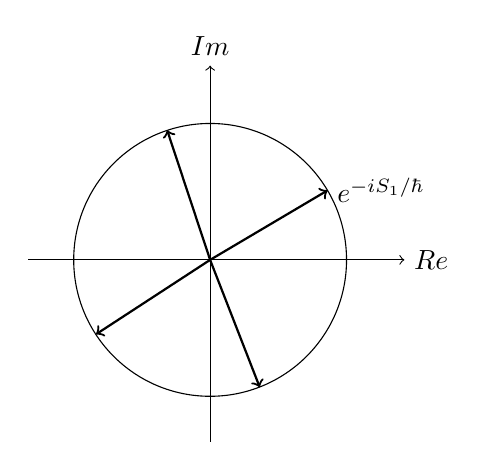
\begin{tikzpicture}[scale=1.05]
\draw[->] (-2.2,0) -- (2.35,0) node[right] {$\operatorname{Re}$};
\draw[->] (0,-2.2) -- (0,2.35) node[above] {$\operatorname{Im}$};
\draw (0,0) circle (1.65);
\draw[thick,->] (0,0) -- (1.42,0.84);
\draw[thick,->] (0,0) -- (-1.38,-0.90);
\draw[thick,->] (0,0) -- (-0.52,1.57);
\draw[thick,->] (0,0) -- (0.60,-1.54);
\node[right] at (1.42,0.84) {$e^{-iS_1/\hbar}$};
\end{tikzpicture}
\caption{Las fases de módulo unidad pueden cancelarse cuando sus direcciones difieren.}
\end{figure}

En efecto,
\begin{equation}
e^{-iS/\hbar}
=
\cos\!\left(\frac{S}{\hbar}\right)
-i\sin\!\left(\frac{S}{\hbar}\right).
\end{equation}
Cada contribución es un vector unitario. Las contribuciones que apuntan en direcciones distintas se restan además de sumarse. Cerca de un punto estacionario de \(S\), las historias próximas tienen fases casi iguales, así que sus contribuciones se refuerzan con más eficacia. Lejos de la acción estacionaria, la fase varía rápidamente y predomina la interferencia destructiva.

Esta estructura de integral de camino sustenta prácticamente toda la teoría cuántica de campos moderna. El siguiente paso práctico se enunciará, no se derivará. Es una vía muy simplificada para abordar el cálculo, pero permite ver cómo se puede describir el mismo objeto en dos lenguajes.

Calcular un proceso es calcular una probabilidad de transición entre un estado inicial y uno final. Una descripción especifica una configuración inicial del campo y una configuración final. La otra especifica partículas entrantes y salientes, los cuantos de uno o varios campos. Estas preguntas parecen distintas, pero ambas se calculan a partir de la misma integral de camino de la teoría de campos.

\section{Una formulación discreta del espacio-tiempo}

Para dar un significado concreto a la suma sobre historias de campos, dividimos el espacio-tiempo en celdas pequeñas y asignamos un valor del campo a cada una. El límite continuo se alcanza al reducir el tamaño de las celdas, pero por ahora estas tienen un tamaño finito. Así, la suma formal sobre funciones se convierte en una suma sobre asignaciones de números a las celdas de una retícula.

Una heurística anterior emplea un producto de factores parecidos a \(1+\mathcal{L}_i\), uno por celda, y luego identifica los términos que describen la propagación y la colisión de partículas. La construcción es lo bastante central como para repetirla, pero hay que corregir el factor. La cantidad pequeña no es el lagrangiano mismo, sino la acción contenida en una celda.

Si una celda tiene volumen espacio-temporal
\begin{equation}
a^4=\Delta t\,\Delta x\,\Delta y\,\Delta z,
\end{equation}
su acción es
\begin{equation}
A_i=\mathcal{L}_i a^4.
\end{equation}
Como la celda es pequeña, \(A_i\) también lo es. Suprimamos temporalmente \(\hbar\). El factor elemental corregido es
\begin{equation}
1-iA_i,
\end{equation}
en vez de \(1+\mathcal{L}_i\).

Para cualquier \(\epsilon\) pequeño,
\begin{equation}
1+\epsilon\simeq e^\epsilon,
\end{equation}
ya que
\begin{equation}
e^\epsilon
=1+\epsilon+\frac{\epsilon^2}{2!}
+\frac{\epsilon^3}{3!}+\cdots.
\end{equation}
Así, en estas unidades provisionales, \(1-iA_i\) aproxima \(e^{-iA_i}\) para una celda suficientemente pequeña. Es más sencillo usar desde el principio el factor exponencial exacto.

\begin{classroomqa}
\lecturetimestamp{00:27:57}
\audiencequestion{¿La exponencial requiere un factor de \(\hbar\)?}
\lecturerresponse{Sí. El factor adimensional de la celda es \(1-iA_i/\hbar\) a primer orden, y la exponencial exacta es \(\exp(-iA_i/\hbar)\). Más adelante se pueden adoptar unidades en las que \(\hbar=1\).}
\end{classroomqa}

Al restituir \(\hbar\), el factor intermedio corregido y su forma exponencial son
\begin{equation}
1-\frac{i}{\hbar}A_i
\simeq
\exp\!\left(-\frac{i}{\hbar}A_i\right).
\end{equation}

Para una historia fija, se sustituye la integral espacio-temporal por una suma de acciones de celda:
\begin{equation}
S[\phi]
=\int d^4x\,\mathcal{L}
\;\longrightarrow\;
\sum_i A_i.
\end{equation}
La fase de esa historia pasa a ser
\begin{equation}
\exp\!\left(-\frac{i}{\hbar}\sum_i A_i\right).
\end{equation}
Una exponencial de una suma es un producto de exponenciales:
\begin{equation}
\exp\!\left(-\frac{i}{\hbar}\sum_i A_i\right)
=
\prod_i\exp\!\left(-\frac{i}{\hbar}A_i\right).
\end{equation}
El orden de las operaciones importa. Primero se elige una historia completa y se multiplican sus pesos de celda. Solo entonces se suman las distintas historias.

La retícula también hace explícitos los datos de frontera.\footnote{El damero y sus filas primera y última fijas se reconstruyen a partir de los diagramas de aproximadamente 00:23:54 y 00:30:49.}
\begin{figure}[htbp]
\centering
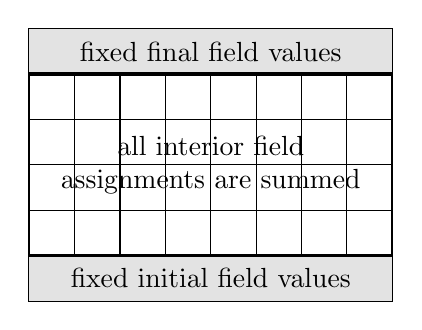
\begin{tikzpicture}[scale=0.72]
\draw[step=0.8,thin] (0,0) grid (6.4,4.8);
\draw[thick] (0,0) rectangle (6.4,4.8);
\fill[gray!22] (0,0) rectangle (6.4,0.8);
\fill[gray!22] (0,4.0) rectangle (6.4,4.8);
\draw[very thick] (0,0.8) -- (6.4,0.8);
\draw[very thick] (0,4.0) -- (6.4,4.0);
\node at (3.2,0.4) {fixed initial field values};
\node at (3.2,4.4) {fixed final field values};
\node[align=center] at (3.2,2.4) {all interior field\\assignments are summed};
\end{tikzpicture}
\caption{Historias discretas del campo con filas inicial y final fijas en la retícula.}
\end{figure}

La primera fila especifica la configuración inicial del campo, y la última, la configuración final. En cada celda interior se permite cualquier valor del campo incluido en la discretización. Por tanto, la amplitud de transición adopta esquemáticamente la forma
\begin{equation}
\mathcal{A}\!\left[\phi_{\mathrm{i}}\rightarrow\phi_{\mathrm{f}}\right]
=
\sum_{\{\phi\}_{\mathrm{interior}}}
\prod_i\exp\!\left(-\frac{i}{\hbar}A_i[\phi]\right),
\end{equation}
con las filas primera y última fijas. Equivalentemente, para cada asignación interior se calcula la exponencial de la acción total y se suma esa contribución a las de todas las demás asignaciones.

\section{De las configuraciones de campo a las configuraciones de partículas}

La misma amplitud de transición puede describirse en términos de campos o de partículas. En lugar de fijar el campo en las hipersuperficies de tiempo inicial y final, se puede especificar un conjunto entrante de cuantos de campo y otro saliente, y luego preguntar por la amplitud que los conecta. El objeto que se evalúa es el mismo. Solo cambia la descripción de frontera.

Los campos cuánticos contienen operadores de creación y aniquilación. Por tanto, los productos de campos actúan sobre los estados de partículas creando, destruyendo o desplazando cuantos. Esta interpretación en términos de operadores es lo que convierte la integral de camino en la retícula en un conjunto de reglas para partículas.

\begin{classroomqa}
\lecturetimestamp{00:34:11}
\audiencequestion{¿Los cuantos de campo son necesariamente identificables como partículas?}
\lecturerresponse{No siempre en el sentido convencional de partículas observables por separado. Por ejemplo, los quarks son cuantos de campos de quarks, pero el confinamiento impide que un quark aislado escape y se detecte por sí solo. En términos más generales, no tiene por qué haber una correspondencia uno a uno entre los campos mencionados en una teoría y las especies de partículas que aparecen como estados observables convencionales. Algunas teorías de campos no admiten esa correspondencia sencilla. Si se usa «``partícula''» en sentido amplio para referirse a un cuanto indivisible que transporta energía y otros números cuánticos, la distinción puede convertirse en parte en una cuestión terminológica.}
\end{classroomqa}

\editorialnote{La cláusula sobre acoplamiento débil de la fuente, entre 00:35:45--00:36:08, es gramaticalmente ambigua y aquí queda sin resolver. La afirmación segura es que las etiquetas de los campos y las especies de partículas observables en el sentido convencional no tienen por qué corresponderse una a una.}

La suma en la retícula sigue abarcando valores del campo. No se restringe a configuraciones que se parezcan a soluciones clásicas suaves.

\begin{classroomqa}
\lecturetimestamp{00:36:44}
\audiencequestion{¿Las historias del campo deben ser continuas, o al menos aproximadamente continuas?}
\lecturerresponse{No. En una retícula discreta, las celdas vecinas simplemente llevan valores del campo, y toda asignación se incluye en la suma. No hay ninguna restricción a historias aproximadamente continuas. Los campos cuánticos fluctúan mucho; las historias típicas no son campos clásicos suaves.}
\end{classroomqa}

Las variables asignadas de forma independiente son los campos en los sitios o celdas de la retícula. Sus derivadas se obtienen mediante diferencias entre valores vecinos.

\begin{classroomqa}
\lecturetimestamp{00:37:56}
\audiencequestion{¿Se asignan valores independientes a los campos y a sus derivadas?}
\lecturerresponse{No. Los valores del campo se asignan en los sitios. Luego se reconstruye una derivada a partir de la diferencia entre valores del campo en sitios vecinos. Hay distintas convenciones para las diferencias finitas, pero las derivadas no son variables independientes adicionales.}
\end{classroomqa}

Así, para un espaciado de retícula \(a\), se puede escribir esquemáticamente
\begin{equation}
\partial_\mu\phi(x)
\longrightarrow
\frac{\phi(x+a\hat\mu)-\phi(x)}{a}.
\end{equation}
El eje de valores del campo también puede dividirse en intervalos pequeños, de modo que queden conjuntos numerables de valores posibles en cada sitio.

\begin{classroomqa}
\lecturetimestamp{00:38:53}
\audiencequestion{¿Qué cambia cuando hay más de un campo?}
\lecturerresponse{Se asigna un valor de cada campo en cada sitio, y la suma abarca todas esas asignaciones.}
\end{classroomqa}

Un campo de valores complejos no debe confundirse con una función analítica de una variable compleja. La analiticidad impone una condición de suavidad excepcionalmente fuerte. Las historias de una integral de camino de campos no tienen por qué satisfacerla y, en general, ni siquiera son aproximadamente suaves.

\begin{classroomqa}
\lecturetimestamp{00:39:07}
\audiencequestion{Si los campos tienen valores complejos, ¿deben estos satisfacer las condiciones de suavidad que cumplen las funciones analíticas?}
\lecturerresponse{No. Tener valores complejos no implica ser analítica. La teoría de funciones analíticas se ocupa de una clase de funciones sumamente suaves y muy restringidas. Las historias del campo que se suman aquí no tienen por qué ser funciones analíticas de la posición; las historias típicas son muy irregulares y, en el límite continuo, pueden considerarse muy discontinuas.}
\end{classroomqa}

El cálculo resultante parece formidable. Incluso después de discretizar el espacio-tiempo y los valores del campo, puede haber un número enorme de asignaciones que muestrear.

\begin{classroomqa}
\lecturetimestamp{00:40:04}
\audiencequestion{¿Cómo sabe un ordenador cuántas asignaciones de la retícula debe muestrear, o cuándo ha convergido el cálculo?}
\lecturerresponse{Esa pregunta pertenece a la teoría gauge en la retícula o, más generalmente, a la teoría cuántica de campos en la retícula. Hoy es una disciplina computacional eficaz. Participé en los comienzos de la formulación de las reglas de la teoría gauge en la retícula, no en el desarrollo posterior de la tecnología informática. Formular las reglas llevó unas tres semanas; desarrollar la tecnología para hacer estos cálculos llevó alrededor de treinta años. Buena parte de la experiencia práctica provino de la mecánica estadística, donde las funciones de partición también se obtienen sumando sobre configuraciones de una retícula---por ejemplo, según esté ocupado o no un sitio de un cristal. Determinar si se han muestreado suficientes configuraciones es una cuestión técnica. Los expertos saben---o creen saber---cuándo está bajo control el cálculo, y los resultados concuerdan con los experimentos.}
\end{classroomqa}

Las reglas conceptuales de la teoría gauge en la retícula se formularon rápidamente; la tecnología necesaria para hacer cálculos con ellas tardó mucho más. El damero no es solo una analogía: también es el punto de partida de un método computacional práctico.

\section{Términos cuadráticos y propagación de partículas}

Volvamos ahora a la interpretación de los campos en términos de operadores. Para dos sitios vecinos \(x\) y \(x'\), el producto
\begin{equation}
\phi(x)\phi(x')
\end{equation}
puede representar, en un elemento de matriz apropiado de una partícula, la aniquilación de una partícula en un sitio y su creación en el otro. Por tanto, en ese sector de una partícula puede representarse como un salto de un enlace. Esta es una interpretación del producto de operadores, pero no la única.

Los términos responsables de esos enlaces son los términos de derivada. Estrictamente hablando, están asociados no a una celda, sino a un par de sitios vecinos. Por ejemplo, una derivada temporal se convierte en
\begin{equation}
\partial_t\phi(t,\mathbf{x})
\longrightarrow
\frac{\phi(t+a,\mathbf{x})-\phi(t,\mathbf{x})}{a},
\end{equation}
y una derivada espacial se trata del mismo modo a lo largo de un enlace espacial.

\begin{classroomqa}
\lecturetimestamp{00:44:39}
\audiencequestion{¿Los lagrangianos que estamos considerando contienen derivadas segundas?}
\lecturerresponse{Las teorías estándar que se consideran aquí están escritas con derivadas primeras. Por tanto, sus versiones en la retícula usan diferencias primeras entre sitios vecinos.}
\end{classroomqa}

Al elevar al cuadrado una diferencia primera aparecen tanto términos en un mismo sitio como un término cruzado entre sitios vecinos:
\begin{align}
\frac{1}{2}\bigl[\phi(x)-\phi(x')\bigr]^2
&=
\frac{1}{2}\phi(x)^2
+\frac{1}{2}\phi(x')^2
-\phi(x)\phi(x').
\end{align}
El término cruzado puede representar el movimiento de un sitio al otro. Los dos cuadrados corresponden a un mismo sitio. Los términos cuadráticos de las derivadas son los términos cinéticos; primero usaremos sus términos cruzados entre sitios vecinos para construir la propagación.

Para aislar la combinatoria, agrupemos los productos entre sitios vecinos en
\begin{equation}
K=\sum_{\langle x,x'\rangle}\phi(x)\phi(x').
\end{equation}
El factor correspondiente en el peso de la integral de camino se escribe esquemáticamente como
\begin{equation}
e^{-iK}.
\end{equation}
\editorialnote{En este factor esquemático de la retícula se omiten las potencias del espaciado de la retícula, \(\hbar\), los signos de la métrica, las constantes de normalización y los coeficientes de los enlaces.}
Su desarrollo es
\begin{equation}
e^{-iK}
=1-iK-\frac{1}{2!}K^2+\frac{i}{3!}K^3+\cdots,
\end{equation}
o, mostrando las sumas sobre los sitios vecinos,
\begin{align}
e^{-iK}
={}&1
-i\sum_{\langle x,x'\rangle}\phi(x)\phi(x')
\nonumber\\
&-\frac{1}{2!}
\sum_{\langle x,x'\rangle}
\sum_{\langle y,y'\rangle}
\phi(x)\phi(x')\phi(y)\phi(y')
+\cdots .
\end{align}
Cada factor selecciona de manera independiente un par de sitios vecinos.

Los diagramas de partículas obedecen una regla que prohíbe los extremos sueltos. Solo se permite un extremo expuesto cuando la condición de frontera inserta explícitamente una partícula en la hipersuperficie inicial o la elimina en la final. Un enlace aislado en el interior tiene extremos sin emparejar y no representa una contribución completa a la transición prescrita. Los extremos internos de los enlaces deben unirse.

Consideremos primero una retícula de solo dos capas temporales. Si el estado inicial inserta una partícula en \(x\) y el estado final la elimina en el punto vecino \(x'\), el término de primer orden puede conectar las inserciones de frontera:
\begin{equation}
x\longrightarrow x',
\qquad
\mathcal{A}_{\text{one link}}\sim -i.
\end{equation}
El coeficiente \(-i\) es solo el coeficiente de este desarrollo esquemático; se sobreentiende que siguen omitidos los factores de la retícula y de normalización.

\begin{classroomqa}
\lecturetimestamp{00:52:16}
\audiencequestion{¿El término de primer orden correspondiente a un enlace contribuye únicamente cuando los sitios inicial y final pertinentes son vecinos?}
\lecturerresponse{Sí. Ese término selecciona un par de sitios vecinos, de modo que solo puede conectar esos sitios de frontera si son vecinos. La propagación a mayor distancia proviene de productos de orden superior.}
\end{classroomqa}

A segundo orden, los dos factores se suman de manera independiente sobre pares de sitios vecinos:
\begin{equation}
K^2
=
\sum_{\langle x,x'\rangle}
\sum_{\langle y,y'\rangle}
\phi(x)\phi(x')\phi(y)\phi(y').
\end{equation}

\begin{classroomqa}
\lecturetimestamp{00:52:40}
\audiencequestion{¿El segundo par de sitios vecinos tiene que estar junto al par seleccionado por el primer factor?}
\lecturerresponse{No. Cada factor selecciona de manera independiente un par de sitios vecinos. Los dos pares pueden compartir un sitio, estar completamente separados o incluso ser el mismo par. La suma incluye todas las posibilidades.}
\end{classroomqa}

Para una partícula que se propaga a través de tres capas temporales, la selección útil de segundo orden comparte un sitio intermedio:
\begin{equation}
\bigl[\phi(x_0)\phi(x_1)\bigr]
\bigl[\phi(x_1)\phi(x_2)\bigr],
\qquad
x_0\longrightarrow x_1\longrightarrow x_2.
\end{equation}
El extremo del primer enlace se une al comienzo del segundo. Solo quedan expuestos los extremos inicial en \(x_0\) y final en \(x_2\), así que el término contribuye a la transición de una partícula requerida. En la exponencial esquemática, su coeficiente es
\begin{equation}
-\frac{1}{2!}.
\end{equation}

Las selecciones también pueden formar saltos separados.\footnote{Los diagramas de enlaces se reconstruyen a partir de la secuencia entre 00:49:18--00:55:12.}
\begin{figure}[htbp]
\centering
\resizebox{\linewidth}{!}{%
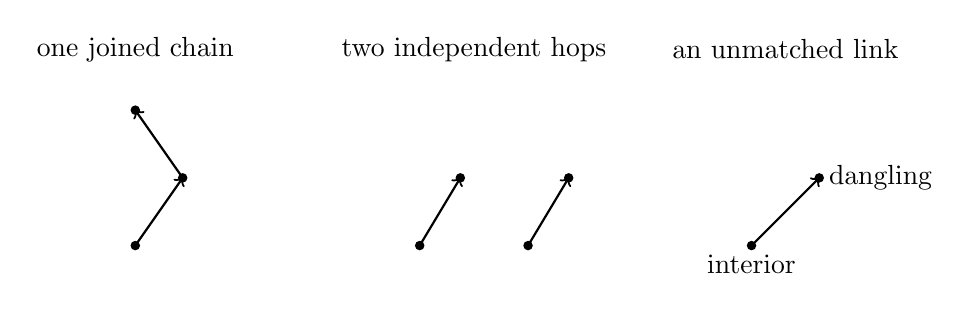
\begin{tikzpicture}[scale=0.86]
\node at (0,2.9) {one joined chain};
\fill (0,0) circle (2pt);
\fill (0.7,1.0) circle (2pt);
\fill (0,2.0) circle (2pt);
\draw[thick,->] (0,0) -- (0.7,1.0);
\draw[thick,->] (0.7,1.0) -- (0,2.0);

\begin{scope}[xshift=4.2cm]
\node at (0.8,2.9) {two independent hops};
\fill (0,0) circle (2pt);
\fill (0.6,1.0) circle (2pt);
\fill (1.6,0) circle (2pt);
\fill (2.2,1.0) circle (2pt);
\draw[thick,->] (0,0) -- (0.6,1.0);
\draw[thick,->] (1.6,0) -- (2.2,1.0);
\end{scope}

\begin{scope}[xshift=9.1cm]
\node at (0.5,2.9) {an unmatched link};
\fill (0,0) circle (2pt);
\fill (1.0,1.0) circle (2pt);
\draw[thick,->] (0,0) -- (1.0,1.0);
\node[below] at (0,0) {interior};
\node[right] at (1.0,1.0) {dangling};
\end{scope}
\end{tikzpicture}%
}
\caption{Selecciones de enlaces vecinos unidos, independientes y sin emparejar.}
\end{figure}

Ya puede haber más de una ruta a este orden. Para un desplazamiento de un paso temporal y uno espacial en la retícula, los dos órdenes
\begin{align}
x
&\longrightarrow x+\hat t
\longrightarrow x+\hat t+\hat s,\\
x
&\longrightarrow x+\hat s
\longrightarrow x+\hat s+\hat t
\end{align}
llegan al mismo extremo.

\begin{classroomqa}
\lecturetimestamp{00:55:53}
\audiencequestion{¿Hay otro camino de dos pasos hasta el mismo extremo diagonal?}
\lecturerresponse{Sí. Se puede dar primero el paso temporal y luego el espacial, o hacerlo en el orden opuesto. Ambas rutas contribuyen a la misma amplitud de transición.}
\end{classroomqa}

No hay motivo para detenerse en dos enlaces. El término de tercer orden aporta cadenas de tres enlaces vecinos. Una ruta puede avanzar directamente, hacer un rodeo o alejarse y volver antes de llegar al punto final. Los órdenes aún superiores incluyen rodeos más largos y retrocesos repetidos. Por tanto, desarrollar la exponencial hasta un orden arbitrario produce una contribución por cada ruta formada por enlaces locales. La amplitud entre dos puntos es la suma de todas ellas, con coeficientes que contienen las potencias correspondientes de \(i\) y factoriales:
\begin{equation}
\begin{gathered}
\mathcal{A}(x_{\mathrm{in}}\to x_{\mathrm{out}})
=
\sum_{\text{joined lattice routes }r}c_r,
\\
c_r\ \hbox{read from the exponential expansion}.
\end{gathered}
\end{equation}
Los coeficientes son, en general, complejos, así que la amplitud resultante también es compleja.

La propagación relativista añade otra posibilidad. Una ruta puede avanzar tanto hacia arriba como hacia abajo en la dirección temporal, y puede recorrer varias veces el mismo enlace.

\begin{classroomqa}
\lecturetimestamp{00:58:47}
\audiencequestion{¿Puede un camino pasar una y otra vez por las mismas dos celdas?}
\lecturerresponse{Sí. Se incluyen los recorridos repetidos y, en el desarrollo relativista, la ruta también puede avanzar hacia atrás en el tiempo.}
\end{classroomqa}

Un segmento que retrocede en el tiempo admite dos interpretaciones gráficas equivalentes. Puede tratarse como una línea de partícula que retrocede en el tiempo. Como alternativa, sigamos el tiempo solo hacia delante: se crea un par partícula--antipartícula, la partícula continúa hacia delante y, más tarde, la antipartícula se encuentra con la partícula original y la aniquila. La misma línea conexa codifica ambas descripciones.\footnote{Las dos interpretaciones siguen el diagrama y la explicación de 005900--005951.}

\begin{figure}[htbp]\centering
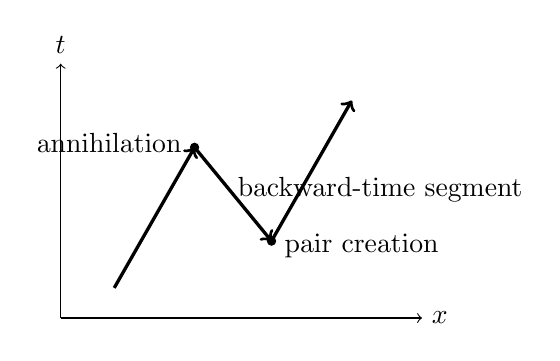
\begin{tikzpicture}[scale=0.85]
\draw[->] (0,0) -- (0,3.8) node[above] {$t$};
\draw[->] (0,0) -- (5.4,0) node[right] {$x$};
\draw[very thick,->] (0.8,0.45) -- (2.0,2.55);
\draw[very thick,->] (2.0,2.55) -- (3.15,1.15);
\draw[very thick,->] (3.15,1.15) -- (4.35,3.25);
\fill (2.0,2.55) circle (2pt);
\fill (3.15,1.15) circle (2pt);
\node[left] at (1.95,2.62) {annihilation};
\node[right] at (3.20,1.08) {pair creation};
\node[right] at (2.50,1.92) {backward-time segment};
\end{tikzpicture}\caption{Un segmento que retrocede en el tiempo, interpretado hacia delante como creación y aniquilación de pares.}\end{figure}

Los factoriales que aparecen en órdenes altos controlan la serie de potencias de la exponencial, pero eso no equivale a controlar la suma completa sobre las configuraciones de campo.

\begin{classroomqa}\lecturetimestamp{01:00:00}\audiencequestion{¿Los factores \(1/n!\) garantizan la convergencia?}\lecturerresponse{Garantizan la convergencia de la serie exponencial para un argumento fijo. Por sí solos, no garantizan la convergencia de la suma separada sobre todas las configuraciones de campo. Son cuestiones distintas. En una red finita con un conjunto finito y discretizado de valores de campo, el número de configuraciones es finito, pero los límites de continuo y de volumen infinito requieren controles adicionales.}\end{classroomqa}

\section{Un producto de enlaces, varias interpretaciones en términos de partículas}

El producto de segundo orden contiene algo más que propagación de una partícula. Cuando los dos pares vecinos comparten un extremo, puede desplazar una partícula a través de una cadena de dos enlaces:
\begin{equation}
\bigl[\phi(x_0)\phi(x_1)\bigr]
\bigl[\phi(x_1)\phi(x_2)\bigr].
\end{equation}
Cuando los pares seleccionados están separados, el mismo término de segundo orden puede desplazar dos partículas, una por cada enlace.\footnote{La comparación entre la propagación de una partícula y dos saltos independientes de un enlace se reconstruye a partir de la discusión en la pizarra de 010046--010234.}
\begin{equation}
\bigl[\phi(x_0)\phi(x_1)\bigr]
\bigl[\phi(y_0)\phi(y_1)\bigr],
\qquad x_0\neq y_0.
\end{equation}
El primer factor transporta una partícula y el segundo transporta otra. Así, la expansión cuadrática en la red contiene amplitudes de propagación en todos los sectores con múltiples partículas. Un mismo orden algebraico puede describir una ruta conexa más larga o varias rutas desconexas más cortas.

Esto contiene muchísima información, pero todavía no constituye un vértice de interacción genuino. Con solo términos cuadráticos de propagación, las líneas conexas de partículas no se dividen para dar un número distinto de líneas. Los procesos que cambian el número de partículas requieren interacciones adicionales, aunque los productos locales de operadores admitan varias interpretaciones en términos de creación y aniquilación.

\begin{classroomqa}\lecturetimestamp{01:03:30}\audiencequestion{¿Podrían aniquilarse un electrón y un positrón y no dejar ninguna partícula?}\lecturerresponse{Una contribución con energía inicial distinta de cero y sin un estado final que transporte energía viola la conservación de la energía. Al sumar las posibles posiciones espaciotemporales, las amplitudes se cancelan. La aniquilación de un electrón--positrón puede ocurrir si otro campo se lleva la energía---por ejemplo, cuando se producen cuantos electromagnéticos.}\end{classroomqa}

\editorialnote{La explicación abreviada pasa directamente de los saltos cuadráticos a la aniquilación de un electrón--positrón. La distinción fundamental es que los términos cuadráticos proporcionan propagación libre, mientras que la aniquilación física requiere una interacción con otro campo; la amplitud sin partículas finales se cancela por conservación de la energía.}

Por tanto, los términos con derivadas hacen mucho, pero no lo hacen todo. Los términos adicionales de la lagrangiana quedan determinados por las propiedades e interacciones de los campos observadas experimentalmente.

\section{El término de masa}

Para un campo escalar, la estructura de derivadas que estamos considerando tiene el siguiente patrón esquemático de signos lorentziano
\begin{equation}
\mathcal{L}_{\mathrm{kin}}
\sim
\frac{1}{2}\left[
(\partial_t\phi)^2
-(\partial_x\phi)^2
-(\partial_y\phi)^2
-(\partial_z\phi)^2
\right].
\end{equation}
Esta expresión fija la estructura temporal menos espacial pertinente para la discusión; los signos globales y las convenciones de normalización quedan implícitos.

La lagrangiana también puede contener potencias del campo sin derivar. El ejemplo cuadrático tiene la forma
\begin{equation}
\text{mass term}\ \propto\ \frac{1}{2}m^2\phi^2,
\end{equation}
donde \(m^2\) se identifica como el coeficiente de masa.\editorialnote{En este pasaje, la fuente no fija la convención de signo global para la lagrangiana escalar completa.} En la interpretación esquemática en términos de partículas, este término aniquila una partícula y la recrea en el mismo sitio de la red. No desplaza la partícula. Inserta un factor en el mismo sitio dentro de una trayectoria:
\begin{equation}
\text{particle at }x
\longrightarrow
\boxed{m^2\phi(x)^2}
\longrightarrow
\text{particle still at }x.
\end{equation}
Cada vez que actúa una inserción de este tipo, la trayectoria adquiere otro factor proporcional a \(m^2\).

Si se conservan únicamente los términos con derivadas, la propagación resultante corresponde a la teoría sin masa en esta expansión esquemática. Para un campo masivo, una ruta puede incluir cualquier número de inserciones de masa en el mismo sitio entre sus términos de salto. El término de masa cambia los pesos relativos de las trayectorias, de modo que el propagador resultante lleva la masa de la partícula.

\section{Términos cúbicos e historias de división--y reunión}

El término de masa cambia el peso de una trayectoria sin mover la partícula. El comportamiento más interesante comienza con términos de grado superior a dos. Consideremos una interacción cúbica,
\begin{equation}
\mathcal{L}_{\mathrm{int}}=g_3\phi^3.
\end{equation}
En una celda de la red, los tres factores de campo admiten cuatro interpretaciones en términos de partículas:
\begin{equation}
1\longrightarrow 2,
\qquad
2\longrightarrow 1,
\qquad
0\longrightarrow 3,
\qquad
3\longrightarrow 0.
\end{equation}
Así, un factor cúbico puede aniquilar una partícula y crear dos, aniquilar dos y crear una, crear tres o aniquilar tres.

Los factores cuadráticos de pares vecinos siguen proporcionando propagación. Una secuencia de ellos puede llevar una partícula hasta una celda; un factor cúbico en esa celda puede absorberla y emitir dos partículas, y más factores cuadráticos pueden llevarse esas dos partículas. Esto contribuye a una amplitud con una partícula entrante y dos salientes.\footnote{La geometría de la red se reconstruye a partir del diagrama de 010848--010942.}

\begin{figure}[htbp]\centering
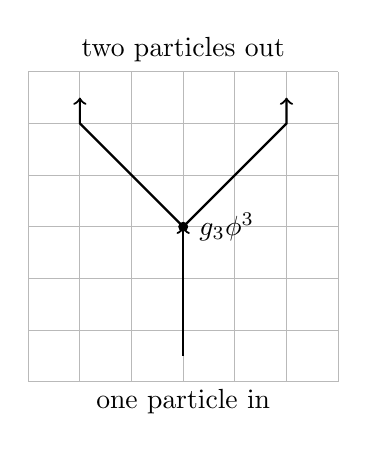
\begin{tikzpicture}[scale=0.82]
\draw[step=0.8,gray!55,thin] (0,0) grid (4.8,4.8);
\draw[thick,->] (2.4,0.4) -- (2.4,1.2) -- (2.4,2.0) -- (2.4,2.4);
\fill (2.4,2.4) circle (2.2pt);
\draw[thick,->] (2.4,2.4) -- (1.6,3.2) -- (0.8,4.0) -- (0.8,4.4);
\draw[thick,->] (2.4,2.4) -- (3.2,3.2) -- (4.0,4.0) -- (4.0,4.4);
\node[right] at (2.5,2.4) {$g_3\phi^3$};
\node at (2.4,-0.3) {one particle in};
\node at (2.4,5.15) {two particles out};
\end{tikzpicture}\caption{Los factores cuadráticos propagan una partícula hasta un vértice cúbico de división y desde él.}\end{figure}

Incluso una amplitud con una partícula tanto al inicio como al final ya no es simplemente una suma de rutas únicas e ininterrumpidas. Una contribución es la propagación directa mediante una cadena de saltos cuadráticos. Otra contiene dos factores cúbicos: la partícula se divide en dos y, más tarde, ambas se reúnen. Por tanto, el estado intermedio puede contener más partículas que el estado externo.\footnote{Las dos alternativas se reconstruyen a partir del diagrama de 010944--011136.}

\begin{figure}[htbp]\centering
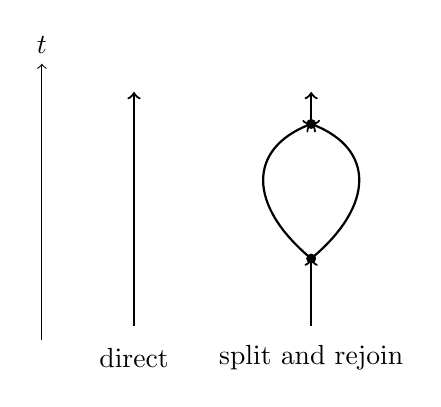
\begin{tikzpicture}[scale=0.9]
\draw[->] (-0.7,0) -- (-0.7,3.9) node[above] {$t$};
\draw[thick,->] (0.6,0.2) -- (0.6,3.5);
\node at (0.6,-0.25) {direct};
\draw[thick,->] (3.1,0.2) -- (3.1,1.15);
\fill (3.1,1.15) circle (2pt);
\draw[thick,->] (3.1,1.15) .. controls (2.2,1.9) and (2.2,2.7) .. (3.1,3.05);
\draw[thick,->] (3.1,1.15) .. controls (4.0,1.9) and (4.0,2.7) .. (3.1,3.05);
\fill (3.1,3.05) circle (2pt);
\draw[thick,->] (3.1,3.05) -- (3.1,3.5);
\node at (3.1,-0.25) {split and rejoin};
\end{tikzpicture}\caption{Propagación directa y contribución con división--y reunión a una misma amplitud de una partícula.}\end{figure}

En electrodinámica, el ejemplo correspondiente es un electrón que emite un fotón y luego lo reabsorbe. Esa historia de emisión y reabsorción forma parte de la amplitud de propagación del electrón de un punto a otro. Los órdenes superiores contienen varias emisiones y absorciones. Un fotón puede convertirse en un par electrón--positrón, y el electrón y el positrón de ese par intermedio pueden intercambiar a su vez un fotón. No hay ninguna razón para que el contenido de partículas intermedio sea sencillo solo porque el contenido inicial y final de partículas lo sea.\footnote{Los ejemplos de la reconstrucción siguiente aparecen en 011122--011234.}

\begin{figure}[htbp]\centering
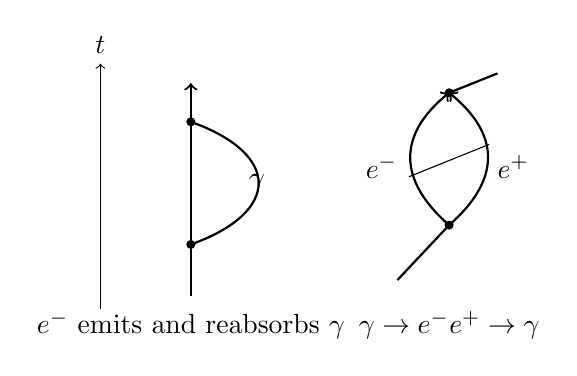
\begin{tikzpicture}[scale=0.82]
\draw[->] (-0.6,0) -- (-0.6,3.8) node[above] {$t$};
\draw[thick,->] (0.8,0.2) -- (0.8,3.5);
\fill (0.8,1.0) circle (2pt);
\fill (0.8,2.9) circle (2pt);
\draw[thick] (0.8,1.0) .. controls (2.2,1.5) and (2.2,2.4) .. (0.8,2.9);
\node[right] at (1.55,1.95) {$\gamma$};
\node at (0.8,-0.25) {$e^-$ emits and reabsorbs $\gamma$};
\draw[thick] (4.0,0.45) -- (4.8,1.3);
\fill (4.8,1.3) circle (2pt);
\draw[thick,->] (4.8,1.3) .. controls (4.0,2.0) and (4.0,2.7) .. (4.8,3.35);
\draw[thick,->] (4.8,1.3) .. controls (5.6,2.0) and (5.6,2.7) .. (4.8,3.35);
\fill (4.8,3.35) circle (2pt);
\draw[thick] (4.8,3.35) -- (5.55,3.65);
\draw[thin] (4.18,2.05) -- (5.42,2.55);
\node[left] at (4.15,2.2) {$e^-$};
\node[right] at (5.4,2.2) {$e^+$};
\node at (4.8,-0.25) {$\gamma\to e^-e^+\to\gamma$};
\end{tikzpicture}\caption{Una contribución de autoemisión del electrón y una historia del fotón que contiene un par electrón--positrón.}\end{figure}

Cada historia de este tipo procede de un producto definido de términos de la expansión de la exponencial. Su coeficiente lleva la potencia correspondiente de \(i\), un factorial procedente de la serie exponencial y los acoplamientos asociados a sus vértices. El coeficiente da la contribución de esa historia, pero la amplitud para los estados inicial y final especificados es la suma de todas las historias con esos mismos estados externos.

\begin{classroomqa}\lecturetimestamp{01:13:18}\audiencequestion{¿Puede el mismo proceso global ocurrir mediante varias historias distintas, todas las cuales contribuyan a su amplitud?}\lecturerresponse{Sí. La amplitud del proceso se obtiene sumando todas las historias distintas que conectan el mismo estado inicial con el mismo estado final.}\end{classroomqa}

Por tanto, hay dos maneras equivalentes de organizar la teoría cuántica de campos. En la descripción de campos, se especifican una configuración inicial y otra final del campo, y se suman todas las historias de campo intermedias. En la descripción de partículas, el campo se descompone en cuantos: se especifican el contenido de partículas entrantes y el de partículas salientes, y se suman todas las historias de partículas que los conectan. La misma lagrangiana rige ambas descripciones.

\section{Términos cuárticos, leyes de conservación y acoplamientos}

Una interacción cuártica,
\begin{equation}
\mathcal{L}_{\mathrm{int}}=g_4\phi^4,
\end{equation}
tiene cuatro factores de campo en un punto. Sus interpretaciones locales en términos de partículas incluyen
\begin{equation}
\begin{gathered}
2\longrightarrow2,
\qquad
1\longrightarrow3,
\qquad
3\longrightarrow1,\\
0\longrightarrow4,
\qquad
4\longrightarrow0.
\end{gathered}
\end{equation}
Por tanto, un único vértice de cuatro patas puede describir la dispersión de dos partículas, la división de una partícula en tres, la unión de tres en una o las cuatro patas orientadas hacia fuera o hacia dentro.\footnote{Las orientaciones se reconstruyen a partir del diagrama de 011428--011518.}

\begin{figure}[htbp]\centering
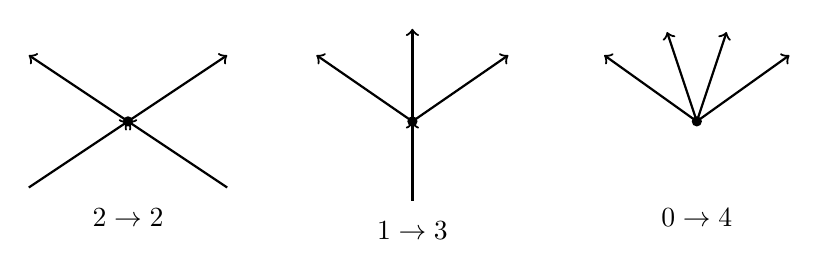
\begin{tikzpicture}[scale=0.84]
\fill (0,0) circle (2.2pt);
\draw[thick,->] (-1.5,-1.0) -- (0,0);
\draw[thick,->] (1.5,-1.0) -- (0,0);
\draw[thick,->] (0,0) -- (-1.5,1.0);
\draw[thick,->] (0,0) -- (1.5,1.0);
\node at (0,-1.45) {$2\to2$};
\begin{scope}[xshift=4.3cm]
\fill (0,0) circle (2.2pt);
\draw[thick,->] (0,-1.2) -- (0,0);
\draw[thick,->] (0,0) -- (-1.45,1.0);
\draw[thick,->] (0,0) -- (0,1.4);
\draw[thick,->] (0,0) -- (1.45,1.0);
\node at (0,-1.65) {$1\to3$};
\end{scope}
\begin{scope}[xshift=8.6cm]
\fill (0,0) circle (2.2pt);
\draw[thick,->] (0,0) -- (-1.4,1.0);
\draw[thick,->] (0,0) -- (-0.45,1.35);
\draw[thick,->] (0,0) -- (0.45,1.35);
\draw[thick,->] (0,0) -- (1.4,1.0);
\node at (0,-1.45) {$0\to4$};
\end{scope}
\end{tikzpicture}\caption{Tres orientaciones locales de un vértice de interacción de cuatro patas.}\end{figure}

La interpretación local \(0\to4\) no significa por sí sola que cuatro partículas puedan aparecer del vacío como un proceso físico. Aún hay que sumar el vértice sobre todas las posiciones espaciotemporales posibles. Cuando el estado externo propuesto no puede conservar la energía, las fases correspondientes a esas posiciones se cancelan.

\begin{classroomqa}\lecturetimestamp{01:15:18}\audiencequestion{¿Describe la orientación con las cuatro patas hacia fuera la aparición espontánea de cuatro partículas en el estado final?}\lecturerresponse{Es una interpretación local del operador de cuatro campos, pero un proceso sin energía entrante viola la conservación de la energía. Al sumar las amplitudes correspondientes a todas las posiciones espaciotemporales posibles del vértice, se cancelan y dan cero.}\end{classroomqa}

\begin{classroomqa}\lecturetimestamp{01:15:58}\audiencequestion{¿Surgen del propio cálculo la conservación de la energía y la conservación del momento?}\lecturerresponse{Sí. La integración del vértice sobre todo el tiempo impone la conservación de la energía, y su integración sobre todo el espacio impone la conservación del momento. La suma sobre las posiciones del vértice se anula a menos que se conserven ambas magnitudes.}\end{classroomqa}

Sujeto a esas leyes de conservación, todo diagrama permitido por la lagrangiana aporta cierta amplitud. La magnitud de esa contribución depende, en parte, del coeficiente de cada término de interacción. Denotemos los coeficientes cúbico y cuártico por \(G_3\) y \(G_4\). Cada vértice de tres patas aporta un factor de \(G_3\), y cada vértice de cuatro patas, un factor de \(G_4\). Por tanto, un diagrama con \(V_3\) vértices cúbicos y \(V_4\) vértices cuárticos tiene esquemáticamente la dependencia de acoplamiento
\begin{equation}
\mathcal{A}_{\mathrm{graph}}
\propto G_3^{V_3}G_4^{V_4}.
\end{equation}

Si estos acoplamientos son pequeños, en general un diagrama con pocos vértices aporta más que uno con muchos. Cada vértice adicional introduce otro factor pequeño. Esto da a la suma perturbativa la posibilidad de ser útil: se empieza con los diagramas más sencillos y luego se añaden correcciones sucesivamente menores.

Determinar si la serie completa converge realmente es una cuestión difícil. Los acoplamientos pequeños hacen plausible ese ordenamiento, pero por sí solos no resuelven todos los problemas de convergencia. Para acoplamientos grandes, la serie ingenua puede fallar por completo. Ese fallo no demuestra que la teoría subyacente sea incorrecta; puede indicar únicamente que la expansión en potencias del acoplamiento era una forma poco adecuada de calcularla. Los métodos que estamos tratando son más directamente útiles cuando los acoplamientos son lo bastante pequeños como para que un diagrama con cuatro vértices sea mucho menor que uno con dos.

\begin{classroomqa}\lecturetimestamp{01:19:24}\audiencequestion{¿Puede tratarse la teoría del color de la misma manera?}\lecturerresponse{Sí. La teoría del color puede formularse de la misma manera y se tratará más adelante.}\end{classroomqa}

\section{Propagadores, vértices y descripciones complementarias}

La siguiente tarea es enumerar las partículas y codificar su dinámica mediante una lagrangiana o mediante reglas de Feynman. Son dos formas de expresar la misma información. Los términos cuadráticos describen la propagación de un punto a otro. Una línea que representa esa propagación se llama propagador. Los términos que incluyen tres campos o más describen lugares donde se encuentran las líneas. Esos puntos de encuentro son los vértices. Por ejemplo,
\begin{equation}
\begin{aligned}
\text{quadratic term}
&\longleftrightarrow \text{propagator},\\
G_3\phi^3
&\longleftrightarrow \text{three-leg vertex}.
\end{aligned}
\end{equation}

Se puede especificar una teoría dando un campo cuántico para cada partícula y escribiendo una lagrangiana que contenga todas sus masas e interacciones. De manera equivalente, se pueden enumerar todos los propagadores, todos los vértices permitidos y el coeficiente asociado a cada vértice. Cualquiera de las dos listas indica qué procesos son posibles y cómo asignar amplitudes a sus diagramas.

Por ejemplo, dos electrones pueden dispersarse mediante el intercambio de un fotón. Cada línea electrónica contiene un vértice electrón--electrón--fotón, y el propagador del fotón conecta los dos vértices.\footnote{El diagrama se reconstruye a partir del ejemplo de 012138.}

\begin{figure}[htbp]\centering
\begin{tikzpicture}[scale=0.95]
\draw[->] (-0.6,-0.2) -- (0.2,1.4);
\draw[->] (0.2,1.4) -- (-0.7,3.1);
\draw[->] (3.5,-0.2) -- (2.7,1.4);
\draw[->] (2.7,1.4) -- (3.6,3.1);
\fill (0.2,1.4) circle (2pt);
\fill (2.7,1.4) circle (2pt);
\draw[thick] (0.2,1.4) -- (2.7,1.4);
\node[above] at (1.45,1.4) {$\gamma$};
\node[left] at (-0.2,0.5) {$e^-$};
\node[right] at (3.1,0.5) {$e^-$};
\end{tikzpicture}\caption{Dispersión de dos electrones mediante el intercambio de un fotón.}\end{figure}

La lagrangiana determina la amplitud de este diagrama y contiene las simetrías y leyes de conservación que la restringen. En un dibujo orientado temporalmente, las partículas situadas abajo forman la configuración inicial y las situadas arriba forman la configuración final.

\begin{classroomqa}\lecturetimestamp{01:22:06}\audiencequestion{En un diagrama de Feynman, ¿las partículas de abajo forman la configuración inicial y las de arriba la configuración final?}\lecturerresponse{Sí. Abajo está la configuración inicial de partículas y arriba, la configuración final.}\end{classroomqa}

Las descripciones en términos de partículas y de campos son complementarias, de manera similar a las descripciones en términos de momento y posición en la mecánica cuántica ordinaria. Describen el mismo sistema en bases distintas. También hay una incertidumbre correspondiente: si el número de partículas está especificado con precisión, el valor del campo es incierto; si el valor del campo está especificado con precisión, el número de partículas es incierto. Ninguna descripción sustituye a la otra, y la lagrangiana es útil en ambas.

\begin{classroomqa}\lecturetimestamp{01:23:26}\audiencequestion{¿Predice la teoría las constantes de acoplamiento o se determinan experimentalmente?}\lecturerresponse{A veces, las simetrías pueden relacionar entre sí distintas constantes de acoplamiento, pero sus valores numéricos suelen proceder de los experimentos.}\end{classroomqa}

\section{Datos experimentales y predicciones de amplio alcance}

La teoría cuántica de campos tiene elegancia y belleza. Pero, al empezar a enumerar los datos---qué partículas hay, cuáles son sus masas y cuáles son sus constantes de acoplamiento---, la lista resulta caótica. Es un caos muy desagradable, con muy poca coherencia aparte de la que aportan las simetrías. Las simetrías relacionan distintos tipos de partículas y sus procesos, pero solo hasta cierto punto. Gran parte del inventario sigue siendo una amplia colección de datos relativamente inconexos sobre un conjunto de tipos de partículas cuya variedad parece tener poca motivación.

\begin{classroomqa}\lecturetimestamp{01:24:58}\audiencequestion{¿Por qué se puede confiar tanto en las constantes de acoplamiento medidas?}\lecturerresponse{Una vez medido un acoplamiento, cambiarlo produce predicciones incorrectas. Su valor queda puesto a prueba por los numerosos cálculos que lo utilizan.}\end{classroomqa}

Hay demasiadas partículas, lo que significa que hay demasiados campos---; demasiados para cualquier sentido estético. Hay aproximadamente un centenar. Hay muchas constantes de acoplamiento, más o menos números extraídos de los experimentos, y muchas masas, que abarcan un rango muy amplio. Hay algunas relaciones entre ellas, pero solo unas pocas.

Pero, una vez que se conocen, se puede empezar a calcular. Una vez conocidas, eso es todo: se puede calcular con gran precisión cualquier cosa sobre esas partículas. Todo lo relativo a los quarks, los electrones, los fotones y los demás alcanza la física atómica, la física de partículas, la física nuclear, la química y quizá la biología. La cantidad de datos de entrada puede ser mayor de lo deseable, pero la cantidad de resultados es enorme.

\section{La electrodinámica cuántica como ejemplo perturbativo}

La electrodinámica cuántica ofrece un ejemplo concreto de la expansión en el acoplamiento.

\begin{classroomqa}\lecturetimestamp{01:26:12}\audiencequestion{Para electrones y fotones, ¿cuántos acoplamientos de interacción del tipo \(G_n\) hay?}\lecturerresponse{Hay un único acoplamiento de interacción elemental: la carga eléctrica \(e\). Es un coeficiente del tipo \(G_3\) asociado a un vértice donde entra un electrón, sale un electrón y se emite o absorbe un fotón.}\end{classroomqa}

Si omitimos las matrices y los índices espinoriales, el contenido esquemático de campos de la interacción es
\begin{equation}
\mathcal{L}_{\mathrm{QED,int}}
\sim e\,(\text{electron bilinear})\,A,
\end{equation}
donde \(A\) denota el campo del fotón. La estructura detallada de matrices de Dirac no es necesaria para el argumento de recuento. La regla elemental de la electrodinámica cuántica es que un electrón emita o absorba un fotón; todos los diagramas más complicados de la electrodinámica cuántica se construyen mediante usos repetidos de ese único vértice.\footnote{El vértice esquemático se reconstruye a partir de 012642; en la fuente se omite deliberadamente la estructura matricial detallada.}

\begin{figure}[htbp]\centering
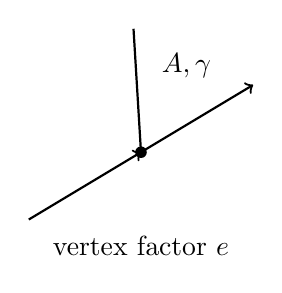
\begin{tikzpicture}[scale=0.95]
\draw[thick,->] (-1.5,-0.9) -- (0,0);
\draw[thick,->] (0,0) -- (1.5,0.9);
\draw[thick] (0,0) -- (-0.1,1.65);
\fill (0,0) circle (2.2pt);
\node[right] at (0.15,1.15) {$A,\gamma$};
\node at (0,-1.25) {vertex factor $e$};
\end{tikzpicture}\caption{El vértice elemental electrón--electrón--fotón de la electrodinámica cuántica.}\end{figure}

\begin{classroomqa}\lecturetimestamp{01:27:38}\audiencequestion{¿Qué ocurre con la dispersión electrón--protón?}\lecturerresponse{En el tratamiento atómico elemental, el protón puede idealizarse como una fuente puntual fija de masa infinita---una partícula pesada clavada en su sitio. Su propia dinámica de campo cuántico solo entra en juego cuando se incluye la teoría interna de los protones y los neutrones.}\end{classroomqa}

\begin{classroomqa}\lecturetimestamp{01:28:30}\audiencequestion{¿Puede el electrón moverse casi a la velocidad de la luz con respecto a ese protón?}\lecturerresponse{Sí.}\end{classroomqa}

Consideremos la dispersión de un fotón por un electrón. En el orden más bajo, el diagrama tiene dos vértices electrón--electrón--fotón. Por tanto, la amplitud es proporcional a \(e^2\):
\begin{equation}
\mathcal{A}_{\mathrm{lowest}}\propto e^2.
\end{equation}
La probabilidad, o, de manera equivalente, la dependencia de la sección eficaz con el acoplamiento, se obtiene del módulo al cuadrado y es proporcional a \(e^4\):
\begin{equation}
P_{\mathrm{lowest}}\ \text{or}\ \sigma_{\mathrm{lowest}}
\propto e^4.
\end{equation}
Con la normalización adimensional convencional, el acoplamiento eléctrico es pequeño, por lo que una dispersión efectiva es mucho menos probable que el simple paso del fotón sin dispersarse.

Ya hay dos diagramas en este orden. En uno de los ordenamientos, el fotón entrante se absorbe y el saliente se emite más tarde. En el otro, el fotón saliente se emite antes de que se absorba el entrante. Contribuyen ambas amplitudes.\footnote{Los dos ordenamientos temporales se reconstruyen a partir de los diagramas de 012842 y 013018.}

\begin{figure}[htbp]\centering
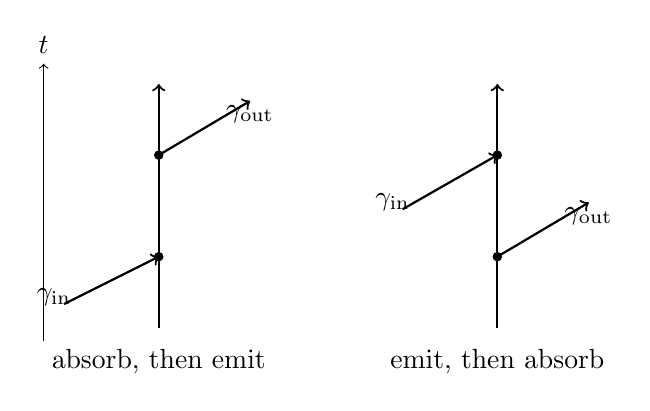
\begin{tikzpicture}[scale=0.86]
\draw[->] (-0.7,0) -- (-0.7,4.1) node[above] {$t$};
\draw[thick,->] (1.0,0.2) -- (1.0,3.8);
\fill (1.0,1.25) circle (2pt);
\fill (1.0,2.75) circle (2pt);
\draw[thick,->] (-0.4,0.55) -- (1.0,1.25);
\draw[thick,->] (1.0,2.75) -- (2.35,3.55);
\node[left] at (-0.15,0.65) {$\gamma_{\mathrm{in}}$};
\node[right] at (1.85,3.35) {$\gamma_{\mathrm{out}}$};
\node at (1.0,-0.3) {absorb, then emit};
\begin{scope}[xshift=5.0cm]
\draw[thick,->] (1.0,0.2) -- (1.0,3.8);
\fill (1.0,1.25) circle (2pt);
\fill (1.0,2.75) circle (2pt);
\draw[thick,->] (1.0,1.25) -- (2.35,2.05);
\draw[thick,->] (-0.4,1.95) -- (1.0,2.75);
\node[right] at (1.85,1.85) {$\gamma_{\mathrm{out}}$};
\node[left] at (-0.15,2.05) {$\gamma_{\mathrm{in}}$};
\node at (1.0,-0.3) {emit, then absorb};
\end{scope}
\end{tikzpicture}\caption{Los dos ordenamientos temporales de orden más bajo para la dispersión electrón--fotón.}\end{figure}

Por consiguiente, la amplitud de orden más bajo no corresponde a un solo diagrama, sino a la suma de los dos:
\begin{equation}
\begin{aligned}
\mathcal{A}^{(2)}
&=
\mathcal{A}_{\mathrm{absorb\ then\ emit}}
+\mathcal{A}_{\mathrm{emit\ then\ absorb}},\\
\mathcal{A}^{(2)}&\propto e^2.
\end{aligned}
\end{equation}

Las correcciones de orden superior añaden más vértices elementales. Un fotón interno adicional unido dos veces a la línea del electrón añade dos factores de \(e\), lo que da una contribución proporcional a \(e^4\) en la amplitud y a \(e^8\) en su módulo al cuadrado. Una línea de fotón también puede contener una inserción de un par electrón--positrón, que añade de nuevo vértices elementales y potencias adicionales de \(e\). Estos son ejemplos, no una lista exhaustiva; el fotón adicional puede acoplarse en muchas posiciones.\footnote{Las estructuras de orden superior se reconstruyen a partir de 013038--013116.}

\begin{figure}[htbp]\centering
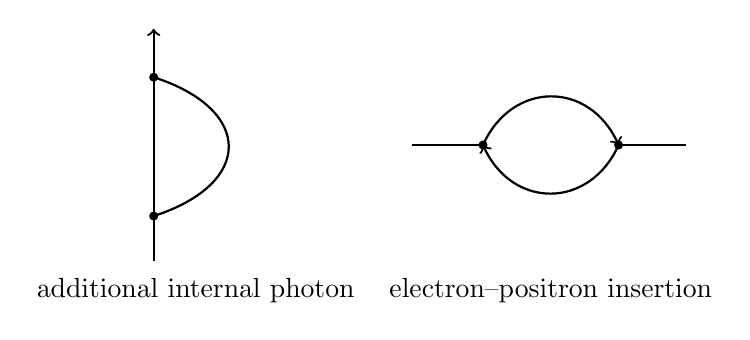
\begin{tikzpicture}[scale=0.82]
\draw[thick,->] (0.9,0.2) -- (0.9,3.8);
\fill (0.9,0.9) circle (2pt);
\fill (0.9,3.05) circle (2pt);
\draw[thick] (0.9,0.9) .. controls (2.45,1.4) and (2.45,2.55) .. (0.9,3.05);
\node at (1.55,-0.25) {additional internal photon};
\begin{scope}[xshift=5.1cm]
\draw[thick] (-0.2,2.0) -- (0.9,2.0);
\fill (0.9,2.0) circle (2pt);
\fill (3.0,2.0) circle (2pt);
\draw[thick,->] (0.9,2.0) .. controls (1.35,3.0) and (2.55,3.0) .. (3.0,2.0);
\draw[thick,->] (3.0,2.0) .. controls (2.55,1.0) and (1.35,1.0) .. (0.9,2.0);
\draw[thick] (3.0,2.0) -- (4.05,2.0);
\node at (1.95,-0.25) {electron--positron insertion};
\end{scope}
\end{tikzpicture}\caption{Dos estructuras de orden superior de la electrodinámica cuántica que añaden vértices elementales y potencias adicionales de \(e\).}\end{figure}

Así, la expansión de la electrodinámica cuántica procede en potencias sucesivas de \(e^2\). Cada complicación nueva de magnitud comparable añade dos potencias de la carga eléctrica a la amplitud. Con la normalización utilizada, eso hace que una corrección de este tipo sea aproximadamente cien o doscientas veces menor en amplitud que el orden anterior. Los diagramas más complicados son progresivamente menos importantes, por lo que la suma perturbativa puede resultar útil.

La probabilidad no se obtiene elevando al cuadrado cada diagrama por separado y sumando después esos cuadrados. Primero se suman todas las amplitudes que contribuyen al mismo proceso externo:
\begin{equation}
\mathcal{A}_{\mathrm{total}}=\sum_r\mathcal{A}_r.
\end{equation}
Solo entonces se calcula
\begin{equation}
P=\left|\mathcal{A}_{\mathrm{total}}\right|^2
=\left|\sum_r\mathcal{A}_r\right|^2.
\end{equation}
Los términos cruzados entre distintos diagramas son términos de interferencia. La regla es sencilla y esencial: primero se suma y luego se eleva al cuadrado.

\section{Hacia el inventario de partículas y el modelo estándar}

Con los propagadores, los vértices, el recuento de acoplamientos y la interferencia ya establecidos, puede comenzar propiamente la descripción de la física de partículas. Se pueden nombrar las partículas, especificar sus masas, escribir las lagrangianas que las rigen, determinadas en parte por la teoría y en parte por los experimentos, y estudiar directamente sus simetrías en esas lagrangianas. El mismo marco conduce luego al modelo estándar y a sus propiedades.

\begin{classroomqa}\lecturetimestamp{01:33:22}\audiencequestion{¿Se podría sustituir el coeficiente de masa constante \(m^2\) por el campo de Higgs?}\lecturerresponse{Sí. Esa es la idea correcta; el mecanismo se tratará más adelante.}\end{classroomqa}

\begin{classroomqa}\lecturetimestamp{01:33:42}\audiencequestion{¿Pueden los puntos vecinos de la red \(x\) y \(x'\) estar en dos tiempos distintos?}\lecturerresponse{Sí. Pueden ser vecinos en la dirección temporal; así se representa la propagación vertical en la red.}\end{classroomqa}

Para puntos vecinos, el cuadrado de la diferencia finita contiene términos tanto en el mismo sitio como entre sitios enlazados:
\begin{equation}
\bigl[\phi(x)-\phi(x')\bigr]^2
=
\phi(x)^2+\phi(x')^2-2\phi(x)\phi(x').
\end{equation}

\begin{classroomqa}\lecturetimestamp{01:33:56}\audiencequestion{¿Qué término representa simplemente una partícula en reposo?}\lecturerresponse{Los términos en el mismo sitio \(\phi(x)^2\) y \(\phi(x')^2\) del cuadrado de la diferencia finita representan la partícula en reposo, mientras que el término cruzado \(\phi(x)\phi(x')\) proporciona la interpretación de movimiento. El término de masa explícito también contribuye factores en el mismo sitio que representan la partícula en reposo.}\end{classroomqa}